\documentclass[12pt]{article}
\usepackage{graphicx}
\usepackage{caption}
\usepackage{subcaption}
\usepackage{tikz}
\usepackage{tcolorbox}
\usepackage{listings}
\usepackage{amsmath}
\usepackage{amssymb}
\usepackage{xcolor}
\usepackage[margin=1cm, top=1.5cm, bottom=1.5cm]{geometry}

\tcbuselibrary{breakable}

\title{\textbf{Gráficas y Juegos: Tarea 02}}
\author{Martínez Méndez Ángel Antonio\\Pinzón Chan José Carlos\\Rendón Ávila Jesús Mateo}
\date{\today}

\begin{document}

\maketitle
\begin{center}
\vspace{3cm}
\includegraphics[width=0.195\textwidth]{Escudo.png}
\hspace{0.5cm}
\includegraphics[width=0.2\textwidth]{logo_ciencias.png}
\end{center}
\begin{center}
    \vspace{1cm}
    Universidad Nacional Autónoma de México\\
    Facultad de Ciencias\\
    Profesor: César Hernández Cruz\\
\end{center}

\newpage

%
% Ejercicio 1
%
\textbf{1.} Sea $D$ una digráfica de orden $n$. Demuestre que si $D$ no tiene ciclos dirigidos,
entonces existe un orden total, $v_1 , . . . , v_n$ de $V_D$ , tal que siempre que $(v_i , v_j)$ sea
una flecha de $D$, se tiene que $i < j$.\\

\begin{tcolorbox}[title=\textbf{Hipotesis}, colback=red!15!white, colframe=black!, breakable]
    $D$ no tiene ciclos dirigidos
\end{tcolorbox}

\begin{tcolorbox}[title=\textbf{Definiciones}, colback=blue!15!white, colframe=black!, breakable]
    $Def$. Un \textbf{ciclo dirigido} de tres o más vértices es una digráfica simple en la que su conjunto
    de vértices admite un orden cíclico de tal forma que dos vértices son adyacentes si y
    sólo si son consecutivos en el orden.
\end{tcolorbox}

Al trabajar en una digráfica acíclica, recordemos que existe por lo menos un vértice con ingrado cero, 
de lo contrario, $D$ sería una digráfica con un ciclo dirigido inducido. Tomaremos a dicho vértice como 
el primero en nuestro orden de vértices debido a que, por definición, no hay ninguna flecha que incida en él. \\

Sea $D$ una digráfica simple, de orden $n$ y acíclica. Si el conjunto de sus vértices esta denotado 
por $V_D$  = \{$v_1, v_2  . . . , v_n$\}, $i.e$, tienen un orden $n$, podemos suponer que  $v_1 \in V_D$
y demostramos por inducción que:\\

$(Base)$ Si $D$ tiene solo un vertice, entonces $v_1 \in V_D$ tiene ingrado $d^-(v_1)$ = 0 y, necesariamente, cumple con ser un orden total.\\

$(Hipotesis Inductiva)$ Supongamos que si $D$ tiene $k$ vertices, existe un orden $k$ de la forma 
$v_1, v_2, \dots, v_k$ tal que si $v_i v_j \in A_D$, por definición sabemos que debe existir $d^-(v_i)$ = 0, que si se cumple, 
podemos eliminar este vertice y la flecha que sale de él y comprobar para los siguientes dos vertices $(v_j v_j+1)$. 
En caso contrario, tendremos que probar esto mismo para los dos vertices anteriores $v_i-1 v_i$.\\

$(Paso inductivo)$ Sea $D$ una digrafica con $k + 1$ vertices.\\

Por definción, debe existir un vertice $v_i \in V_D$ con ingrado cero que cumpla con ser el primero en nuestro orden. Por $H.I.$
si vamos revisando vértice por vértice, si alguno de estos $\{v_i, v_i+1, ..., v_k, v_k+1\}$ cae en tener ingrado $1$ o $0$, llegaremos a nuestro caso base en $v_{k+1}$,
donde tendremos un orden de la forma $v_k < v_i$. 

\vspace{1cm}

%
% Ejercicio 2
%
\textbf{2.} Demuestre que si $G$ tiene diámetro mayor que 3, entonces $\overline{G}$ tiene diámetro menor que 3.

\begin{tcolorbox}[title=\textbf{Hipotesis}, colback=red!15!white, colframe=black!, breakable]
    $G$ tiene un diámetro mayor que 3.
\end{tcolorbox}
\begin{tcolorbox}[title=\textbf{Definiciones}, colback=blue!15!white, colframe=black!, breakable]
    $Def$. El \textbf{diámetro} de una gráfica $G$ se define como $max_{u\in V_G}$\{$max_{v\in V_G}$\{${d(u,v)}$\}\}, en otras palabras, la distancia mas grande entre cualesquiera vértices de $G$.
    \\
    \\
    $Def$.El \textbf{complemento} de una gráfica $G$, denotada como $\overline{G}$, es la gráfica con el conjunto de vértices:
    \[V(\overline{G}) = V(G)\]
    y el conjunto de aristas:
    \[E(\overline{G}) = \{ uv \in V(G) \times V(G) \mid uv \notin E(G)\}\]
\end{tcolorbox}

Sea $G$ un grafica cuyo diámetro es mayor que 3. De antemano podemos descartar que la grafica sea conexa, pues en ese caso su diametro sería igual a 1.\\

Por hipotesis sabemos que existen 2 vértices $u,v\in G$ tales que $d(u,v)$ $\geq 4$. Esto nos indica que no existe una arista entre $u$ y $v$, tampoco existe un vértice adyacente a ambos y mucho menos dos vértices adyacentes entre si y adyacentes a $u$ y a $v$.\\

Si definimos una biparticion (X,Y) en $G$, sabemos que para cualesquiera vértices  $v_i,v_j \in X$ entonces la arista $v_iv_j \notin E_G$. De forma similar, para cualesquiera dos vértices $u_i,u_j \in Y$ ocurre que la arista  $u_iu_j \notin E_G$. En consecuencia, las aristas  $v_iv_j$ y $u_iu_j$ pertenecen al conjunto de aristas de $\overline{G}$. Esto significa que todo vértice $v_i$ en X, si nos situamos en $\overline{G}$, es adyacente a cualquier otro vertice $v_j$ que tambien pertenezca a X y por lo tanto la distancia entre cualesquiera vértices en X y en $\overline{G}$ es 1.\\
	
\begin{figure}[h!]
    \begin{subfigure}{0.5\textwidth}
        \centering
        
\begin{tikzpicture}[scale=1]
            \node (a) at (0,0) [circle,fill,inner sep=1.5pt] {};
            \node (b) at (0,1) [circle,fill,inner sep=1.5pt] {};
            \node (c) at (0,2) [circle,fill,inner sep=1.5pt] {};
            \node (d) at (0,3) [circle,fill,inner sep=1.5pt] {};

        \end{tikzpicture}
        \caption{Biparticion X, situada en $G$}
    \end{subfigure}
    \begin{subfigure}{0.5\textwidth}
        \centering
        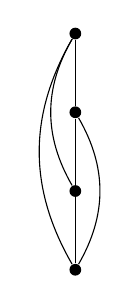
\begin{tikzpicture}[scale=1]
            \node (a) at (0,0) [circle,fill,inner sep=1.5pt] {};
            \node (b) at (0,1) [circle,fill,inner sep=1.5pt] {};
            \node (c) at (0,2) [circle,fill,inner sep=1.5pt] {};
            \node (d) at (0,3) [circle,fill,inner sep=1.5pt] {};
            
            \draw (a) -- (b) (b) -- (c) (c) -- (d);
            \draw (d) to[out=-120,in=120] (a);
            \draw (d) to[out=-120,in=120] (b);
            \draw (c) to[out=-60,in=60] (a);
            
        \end{tikzpicture}
        \caption{Biparticion X, situada en $\overline{G}$}
    \end{subfigure}
\end{figure}

Sean los vértices $v_i \in X$ y $u_j \in Y$, como tenemos una bipartición sabemos que existe al menos una arista que una a algún $v_i$ con algún vértice en Y. Sea uno o multiples elementos en X (no todos) adyacentes a algún $u_j$, entonces habrá un elemento X  tal que no sea adyacente a $u_j$ en G pero si en $\overline{G}$, de modo que (como todos los elementos en $\overline{G}$ y X son adyacentes entre si) puede ser alcanzado y funcionar como "intermediario" para llegar a $u_j$. En este caso la distancia entre los vértices en X y $u_j$ (en el peor de los casos) es 2.\\

Si la gráfica fuera bipartita completa entonces al  aplicar el complemento de G, los vértices en X no podrían alcanzar a los vértices en Y, siendo los vértices en X adyacentes sólo entre ellos, en este otro caso la distancia entre cualesquiera vértices en X es igual a 1. Todo lo anterior es análogo para los vértices en Y.\\

En conclusión,  para todos los casos se cumple que la distancia es menor que 3, por lo tanto el diámetro es menor que 3 y la propiedad se cumple.\\

\vspace{1cm}

%
% Ejercicio 3
%
\textbf{3.} Sea $D$ una digráfica. Utilizando un análogo para digráficas de las matrices de incidencia, dmeuestra que:\\
\[
\sum_{\displaystyle v \in V_D} d^{+}(v) = \sum_{\displaystyle v \in V_D} d^{-}(v) = |A_D|
\]
\begin{tcolorbox}[title=\textbf{Hipotesis}, colback=red!15!white, colframe=black!]
    $D$ es una gŕafica dirigida (digráfica).
\end{tcolorbox}
\begin{tcolorbox}[title=\textbf{Definiciones}, colback=blue!15!white, colframe=black!]
    $Def$. Una gráfica $D$ es una \textbf{gráfica dirigida} si $D$ es una pareja ordenada $D=(V,A)$, donde
    $V$ es un conjunto arbitrario y $A$ es un subconjunto de $V \times V$ (parejas ordenadas).
    \\
    \\
    $Def$. La \textbf{matríz de incidencia} $M$ de $G$ es la matriz de $m \times n$ con entradas en $\{0, 1\}$ tal que:
    \[M_{ij} = \begin{cases} 1 & \text{si el vértice } v_i \in e_j\\ 0 & \text{en otro caso} \end{cases}\]

\end{tcolorbox}

$P.D.$
\[\sum_{\displaystyle v \in V_D} d^{+}(v) = \sum_{\displaystyle v \in V_D} d^{-}(v) = |A_D|\]
Sea $M^+$ y $M^-$ las matrices de incidencia de los exgrados e ingrados respectivamente, si tenemos una gráfica dirigida $D$ y su conjunto
de vértices $V(D)$ tal que:
\[V(D) = \{v_1, v_2, ..., v_n\}\]
y su conjunto de aristas $A(D)$ tal que:
\[A(D) = \{e_1, e_2, ..., e_m\}\]
Para la matríz de incidencia de una digráfica, tanto para los exgrados e ingrados, la suma
de los elementos de cada columna es igual a $1$. Sea la suma de los elementos de la columna igual a $0$,
se concluye que la arista no existe, por otro lado, si la suma es igual a $1$, la arista \textit{sale} de algún vértice (exgrado)
o se dirige a algún vértice (ingrado).\\

Suponiendo que la suma de la columna sea $\geq 2$, esto no es posible puesto que una arista sólo puede partir de un solo punto y viceversa, $i.e$ sólo 
puede dirigirse a un solo punto.\\

Como resultado al sumar todas las columnas de $M^+$ o $M^-$ obtenemos el número de aristas de la gráfica, $i.e$ se obtiene la 
cardinalidad de $A(D)$.

De forma similar, si sumamos las entradas del $i-esimo$ renglón de $M^+$ obtenemos el exgrado (o ingrado en el caso de $M^-$) del vértice $v_i$.\\

En base a lo anterior se puede argumentar que:
\[\mid A(D) \mid = \sum\limits_{j = 1}^{m} 1\]
\[= \sum\limits_{j = 1}^{m} \sum\limits_{n = 1}^{n} M^+_{ij}\]
\[= \sum\limits_{i = 1}^{n} \sum\limits_{j = 1}^{m} M^+_{ij}\]
\[= \sum\limits_{i = 1}^{n} d^+(v_i)\]
\[= \sum\limits_{i = 1}^{n} d^+(v_i)\]
\[= \sum_{\displaystyle v \in V(D)} d^+(v_i)\] 
Analogamente podemos hacerlo para ingrados, por lo que:
\[\mid A(D) \mid = \sum_{\displaystyle v \in V(D)} d^+(v) = \sum_{\displaystyle v \in V(D)} d^-(v)\]



\vspace{1cm}
%
% Ejercicio 4
%
\textbf{4.} Sea $n$ un entero positivo. Definimos la \textit{Retícula Boleana, BL\_n}, como
la gráfica cuyo conjunto de vértices es el conjunto de todos los posibles subconjuntos
de $\{1, ..., n\}$, donde dos subconjuntos $X$ y $Y$ son adyacentes si y sólo si su diferencia
tiene exactamente un elemento.\\
\\
\textbf{(a)} Dibuje $BL_1$, $BL_2$, $BL_3$ y $BL_4$.
\\

Para $BL_1$ tenemos que el conjunto de vértices $V$ es el conjunto de todos los posibles subconjuntos de $\{1\}$, es decir:
\[V(BL_1) = \{\emptyset, \{1\}\}\]

\begin{figure}[h!]
    \centering
    \begin{minipage}{0.4\textwidth}
        \centering
        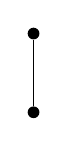
\begin{tikzpicture}[scale=1]
            \node (a) at (0,0) [circle,fill,inner sep=1.5pt] {};
            \node (b) at (0,1) [circle,fill,inner sep=1.5pt] {};

            \draw (a) -- (b);
        \end{tikzpicture}
        \caption{Gráfica de $BL_1$}
    \end{minipage}
\end{figure}

Para $BL_2$ tenemos que el conjunto de vértices $V$ es el conjunto de todos los posibles subconjuntos de $\{1, 2\}$, es decir:
\[V(BL_2) = \{\emptyset, \{1\}, \{2\} \{1, 2\}\}\]

\begin{figure}[h!]
    \centering
    \begin{minipage}{0.4\textwidth}
        \centering
        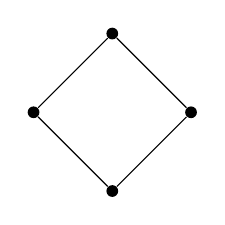
\begin{tikzpicture}[scale=1]
            \node (a) at (1,0) [circle,fill,inner sep=1.5pt] {};
            \node (b) at (0,1) [circle,fill,inner sep=1.5pt] {};
            \node (c) at (2,1) [circle,fill,inner sep=1.5pt] {};
            \node (d) at (1,2) [circle,fill,inner sep=1.5pt] {};

            \draw (a) -- (b) (a) -- (c) (b) -- (d) (c) -- (d);
        \end{tikzpicture}
        \caption{Gráfica de $BL_2$}
    \end{minipage}
\end{figure}

Para $BL_3$ tenemos que el conjunto de vértices $V$ es el conjunto de todos los posibles subconjuntos de $\{1, 2, 3\}$, es decir:
\[V(BL_3) = \{\emptyset, \{1\}, \{2\}, \{3\}, \{1, 2\}, \{1, 3\}, \{2, 3\},\{1, 2, 3\}\}\]

\begin{figure}[h!]
    \centering
    \begin{minipage}{0.4\textwidth}
        \centering
        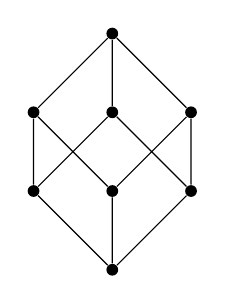
\begin{tikzpicture}[scale=1]
            \node (a) at (1,0) [circle,fill,inner sep=1.5pt] {};
            \node (b) at (0,1) [circle,fill,inner sep=1.5pt] {};
            \node (c) at (1,1) [circle,fill,inner sep=1.5pt] {};
            \node (d) at (2,1) [circle,fill,inner sep=1.5pt] {};
            \node (e) at (0,2) [circle,fill,inner sep=1.5pt] {};
            \node (f) at (1,2) [circle,fill,inner sep=1.5pt] {};
            \node (g) at (2,2) [circle,fill,inner sep=1.5pt] {};
            \node (h) at (1,3) [circle,fill,inner sep=1.5pt] {};

            \draw (a) -- (b) (a) -- (c) (a) -- (d) (b) -- (e) (b) --(f) (c) -- (e) (c) -- (g) (d) -- (f) (d) -- (g) (e) -- (h) (f) -- (h) (g) -- (h);
        \end{tikzpicture}
        \caption{Gráfica de $BL_3$}
    \end{minipage}
\end{figure}

Para $BL_4$ tenemos que el conjunto de vértices $V$ es el conjunto de todos los posibles subconjuntos de $\{1, 2, 3, 4\}$, es decir:
\[V(BL_4) = \{\emptyset, \{1\}, \{2\}, \{3\}, \{4\}, \{1, 2\}, \{1, 3\}, \{1, 4\}, \{2, 3\}, \{2, 4\},\]
\[\{3, 4\}, \\\{1, 2, 3\}, \{1, 3, 4\}, \{1, 2, 4\}, \{2, 3, 4\}, \{1, 2, 3, 4\}\}\]
\newpage
\begin{figure}[h!]
    \centering
    \begin{minipage}{0.4\textwidth}
        \centering
        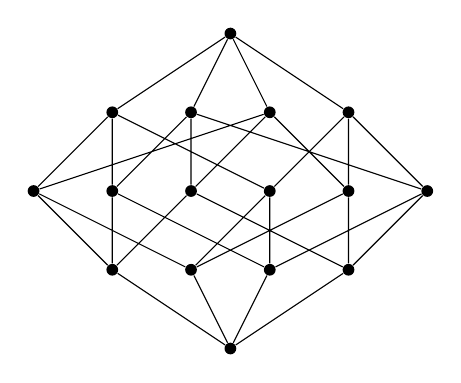
\begin{tikzpicture}[scale=1]
            \node (a) at (2.5,0) [circle,fill,inner sep=1.5pt] {};
            \node (b) at (1,1) [circle,fill,inner sep=1.5pt] {};
            \node (c) at (2,1) [circle,fill,inner sep=1.5pt] {};
            \node (d) at (3,1) [circle,fill,inner sep=1.5pt] {};
            \node (e) at (4,1) [circle,fill,inner sep=1.5pt] {};
            \node (f) at (0,2) [circle,fill,inner sep=1.5pt] {};
            \node (g) at (1,2) [circle,fill,inner sep=1.5pt] {};
            \node (h) at (2,2) [circle,fill,inner sep=1.5pt] {};
            \node (i) at (3,2) [circle,fill,inner sep=1.5pt] {};
            \node (j) at (4,2) [circle,fill,inner sep=1.5pt] {};
            \node (k) at (5,2) [circle,fill,inner sep=1.5pt] {};
            \node (l) at (1,3) [circle,fill,inner sep=1.5pt] {};
            \node (m) at (2,3) [circle,fill,inner sep=1.5pt] {};
            \node (n) at (3,3) [circle,fill,inner sep=1.5pt] {};
            \node (o) at (4,3) [circle,fill,inner sep=1.5pt] {};
            \node (p) at (2.5,4) [circle,fill,inner sep=1.5pt] {};

            \draw (a) -- (b) (a) -- (c) (a) -- (d) (a) -- (e) (b) -- (f) (b) -- (g) (b) -- (h) (c) -- (f) (c) -- (i) (c) -- (j) (d) -- (g) (d) -- (i) (d) -- (k) (e) -- (h) (e) -- (j) (e) -- (k) (f) -- (l) (f) -- (n) (g) --(l) (g) -- (m) (h) -- (m) (h) -- (n) (i) -- (l) (i) -- (o) (j) -- (n) (j) -- (o) (k) -- (m) (k) -- (o) (l) -- (p) (m) -- (p) (n) -- (p) (o) -- (p);
        \end{tikzpicture}
        \caption{Gráfica de $BL_4$}
    \end{minipage}
\end{figure}

\textbf{b)} Determine $|V_{BL_n}|$ y $|E_{BL_n}|$ (Demuestre su respuesta).

\begin{tcolorbox}[title=\textbf{Definiciones}, colback=blue!15!white, colframe=black!]
    $Def$. Sea $A$ un conjunto, definimos al \textbf{conjunto potencia} de $A$, denotado como $\mathcal{P}(A)$, como el conjunto de todos los subconjuntos de $A$. $i.e$:
    \[\mathcal{P}(A) = \{X \mid X \subseteq A\}\]
\end{tcolorbox}
Como sabemos que $V(BL_n)$ es el conjunto de todos los posibles subconjuntos de $\{1, ..., n\}$, entonces
podemos verlo como el conjunto potencia de $\{1, ..., n\}$, es decir:
\[V(BL_n) = \mathcal{P}(\{1, ..., n\})\]
cuya cardinalidad se define como:
\[|V(BL_n)| = 2^n\]

Como ya hemos demostrado $|V(BL_n)| = 2^n$. De tal modo que, para saber $|E(BL_n)|$, nos basaremos en la construcción de aristas en la gráfica $BL_n$\\

Por definición de $BL_n$, sabemos que $u$ es adyacente a $v$ si y sólo si su diferencia simétrica tiene exactamente un elemento.\\

Notemos que, sin importar quien sea $n$, $d(\varnothing) = d(\{1, 2, ... , n\}) = n$ es decir, sus grados son iguales.\\

Así podemos ver al conjunto de vértices de la sigueinte manera:
\[V(BL_n) = \{d(V_1) = n, v_2, ... , d(u) = n \}\]

De esta forma, $| V(BL_n) | = n \times 2^n$

Sin embargo, recordemos que $d(v_i) = n$ solo aplica para los vertices extremos, y con la formula dada, estaríamos asumiendo que todos los vertices de $V(BL_n)$ 
tienen el mismo grado, es decir, estariamos contado dos veces nuestros \textit{"vertices internos"}, tal que: 

\[V(BL_n) = \{ d(v_1) = n, d(v_2) = n, ..., d(u_n) = n \}\]

Así que, solamente dividimos todo nuestra operación entre 2 y tendríamos que $| E(BL_n) | = (n \times 2^n) / 2$
O bien, $| E(BL_n) | = n \times 2^(n - 1)$ Así, nos aseguramos de contar bien los vertices de $BL_n$.\\
 
\textbf{c)} Demuestre que $BL_n$ es bipartita para cualquier $n \in \mathbb{Z} \text{ tal que } n > 0$.

\begin{tcolorbox}[title=\textbf{Definiciones}, colback=blue!15!white, colframe=black!]
    $Def$. Sea $n$ un entero positivo. la \textbf{Retícula Boleana, BL\_n}, como
    la gráfica cuyo conjunto de vértices es el conjunto de todos los posibles subconjuntos
    de $\{1, ..., n\}$, donde dos subconjuntos $X$ y $Y$ son adyacentes si y sólo si su diferencia
    tiene exactamente un elemento.\\

    $Def.$ Una gráfica $G$ es \textbf{bipartita} si $V(G)$ admite una patición $V = (X, Y)$ tal que $X$ y $Y$ son conjuntos independientes.
\end{tcolorbox}

$P.D$ $BL_N$ es bipartita para cualquier $N \in \mathbb{Z^+}$.\\

Sean $u,v$ vertices de $V(BL_n)$. Notemos que por definición, los vértices de $BL_n$  tienen cardinalidad par e impar.\\

Supongamos que tomamos dos vértices pares $u$ y $v$ de nuestra gŕafica $BL_n$, de tal forma que los podemos representar
como $\# u  = 2m$ y $\# v = 2t$ donde $m$ y $t$ son enteros positivos.\\

Digamos que $m > t$ y $m \neq t$ por lo que $m$ es igual a $t + g$, con $g \in \mathbb{N}$. Sin 
importar si hacemos la operación $2 m - 2t$ o $2t - 2m$ tendremos que $2 (t + g) - 2t = 2g$ o $2t - 2(t + g) = 2g$ (por conmutatividad de la suma).\\

Es decir, siempre nos quedara un vértice con cardinalidad par si tratamos de sacar su diferencia simétrica. Analogamente se puede probar lo mismo para los vértices impares.\\

Recordemos que si tenemos un vértice de cardinalidad par o impar estos siempre van a tener al menos una arista por definición de $BL_n$, de 
tal manera que vamos a tener una partición $(X, Y) en V(BL_n)$ tal que $X \cap Y = \varnothing$ \\

Por lo que en nuestro conjunto de vértices $V(BL_n)$ siempre va a existir una bipartición:
\[X = \{ x \mid \# x \text{ es par}\} \text{ y}\]
\[Y = \{ y \mid \# y \text{ es impar}\}\]

De esta manera aseguramos que la gráfica $BL_n$ es bipartita para cualquier $n \in \mathbb{Z^+}$.
\vspace{1cm}

%
% Ejercicio 5
%
\textbf{5.} Caracterice a las gráficas $k$-regulares para $k \in \{0, 1, 2\}$.

\begin{tcolorbox}[title=\textbf{Definiciones}, colback=blue!15!white, colframe=black!]
    $Def$. Una gráfica $G$ es $k$-regular si $d(v) = k$ para cada $v \in V(G)$
\end{tcolorbox}

\textbf{a) Para $k = 0$}\\

Una gráfica $G$ es $0$-regular si y sólo si $G$ es vacia.\\

$\Longrightarrow)$ Sea $G$ una gráfica $0$-regular, entonces $d(v) = 0$ para cada $v \in V(G)$.\\

De lo anterior deducimos que cada vértice $v$ en el conjunto de vértices $V(G)$ no es extremo 
de ninguna arista, $i.e$ $E(G) = \varnothing$.\\

Por lo tanto $G$ es vacia.\\

$\Longleftarrow)$ Sea $G$ una gráfica vacia, entonces $E(G) = \varnothing$, entonces no hay aristas entre vertices.\\

Por lo tanto $d(v) = 0$ para todo $v \in V(G)$, así $G$ es $0$-regular\\

\begin{figure}[h!]
    \centering
    \begin{minipage}{0.6\textwidth}
        \centering
        \begin{tikzpicture}[scale=1]
            \node (a) at (1,0) [circle,fill,inner sep=1.5pt] {};
            \node (b) at (0,1) [circle,fill,inner sep=1.5pt] {};
            \node (c) at (2,1) [circle,fill,inner sep=1.5pt] {};
            \node (d) at (1,2) [circle,fill,inner sep=1.5pt] {};

        \end{tikzpicture}
        \caption{Representación de una gráfica $0$-regular}
    \end{minipage}
\end{figure}

\textbf{b) Para $k = 1$}\\

Una gráfica $G$ es $1$-regular si y solo si $G$ es una gráfica $nK_2$ con $n \in \mathbb{N}$\\

$\Longrightarrow)$ Sea $G$ una gráfica $1$-regular, entonces $d(v) = 1$ para cada $v \in V(G)$.\\

De lo anterior deducimos que para cada vértice $v$ existe un único vértice $u$ tal que $uv \in E(G)$, 
es decir, $G$  es una gráfica $K_2$ cuando $n = 1$.\\

Cuando $n > 1$, entonces por ser $G$ $1$-regular, $G$ es la unión de las $n$ gráficas $K_2$.\\

$\Longleftarrow)$ Sea $G$ una gráfica $nK_2$, entonces $G$ es una gráfica generada por la unión 
de las $n$ gráficas completas de dos vértices.\\

Como $G$ es la unión de las $n$ gráficas $K_2$, podemos decir que para todo $v \in V(G)$, se cumple que $d(v) = 1$.\\

Por lo tanto $G$ es $1$-regular.\\

\begin{figure}[h!]
    \centering
    \begin{minipage}{0.6\textwidth}
        \centering
        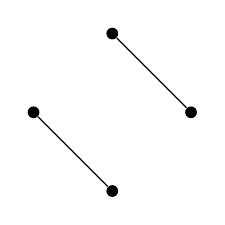
\begin{tikzpicture}[scale=1]
            \node (a) at (1,0) [circle,fill,inner sep=1.5pt] {};
            \node (b) at (0,1) [circle,fill,inner sep=1.5pt] {};
            \node (c) at (2,1) [circle,fill,inner sep=1.5pt] {};
            \node (d) at (1,2) [circle,fill,inner sep=1.5pt] {};

            \draw (a) -- (b) (c) -- (d) ;

        \end{tikzpicture}
        \caption{Representación de una gráfica $1$-regular}
    \end{minipage}
\end{figure}

\textbf{c) Para $k = 2$} \\

Una Grafica $G$ es $2$-regular si y sólo si cada vértice de $G$ tiene exactamente 2 \textit{vecinos}.\\

$\Longrightarrow)$ Sea $G$ una gráfica $2$-regular, entonces $d(v) = 2$ para cada $v \in V(G)$.\\

Como por ser $d(v) = 2$, no puede pasar que $v$ sea adyacente a un vértice $u$ y no sea adyacente 
a algún otro vértice $w$, por lo que todo vértice $v \in V(G)$ deber ser adyacente a algún otro vértice $u$ y $w$
de forma que $uv \in E(G)$ y $vw \in E(G)$.\\

por lo tanto $\forall v \in V(G)$, se cumple $v$ tiene exactamente 2 vecinos.\\

$\Longleftarrow)$ sea $G$ una gráfica tal que cada vértice de $G$ tiene exactamente 2 vecinos.\\

Como cada vértice $v \in V(G)$ tiene exactamente 2 vecinos, entonces $d(v) = 2$ para todo $v \in V(G)$.\\

Por lo tanto $G$ es $2$-regular.\\

\begin{figure}[h!]
    \centering
    \begin{minipage}{0.6\textwidth}
        \centering
        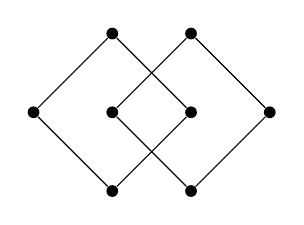
\begin{tikzpicture}[scale=1]
            \node (a) at (1,0) [circle,fill,inner sep=1.5pt] {};
            \node (b) at (0,1) [circle,fill,inner sep=1.5pt] {};
            \node (c) at (1,2) [circle,fill,inner sep=1.5pt] {};
            \node (d) at (2,1) [circle,fill,inner sep=1.5pt] {};
            \node (e) at (2,0) [circle,fill,inner sep=1.5pt] {};
            \node (f) at (1,1) [circle,fill,inner sep=1.5pt] {};
            \node (g) at (2,2) [circle,fill,inner sep=1.5pt] {};
            \node (h) at (3,1) [circle,fill,inner sep=1.5pt] {};


            \draw (a) -- (b) (b) -- (c) (c) -- (d) (a) -- (d) (e) -- (f) (f) -- (g) (g) -- (h) (e) -- (h);

        \end{tikzpicture}
        \caption{Representación de una gráfica $2$-regular}
    \end{minipage}
\end{figure}

%
% Ejercicio 6 
%
\textbf{6.} Demuestre que si $\mid E \mid \geq\mid V \mid$, entonces G contiene un ciclo.

\begin{tcolorbox}[title=\textbf{Hipotesis}, colback=red!15!white, colframe=black!, breakable]
    $\mid E \mid \geq \mid V \mid$.
\end{tcolorbox}

\begin{tcolorbox}[title=\textbf{Definiciones}, colback=blue!15!white, colframe=black!]
    $Def$. Un \textbf{ciclo} de tres o mas vértices es una gráfica simple en la que su conjunto de
    vértices admite un orden cíclico de tal forma que dos vértices son adyacentes si y sólo si son consecutivos en el orden.\\

    $Def$ Una gráfica es \textbf{regular} si es $k$-regular para algún $k \in \mathbb{N}$.
\end{tcolorbox}

$Dem.$ $por$ $casos$\\

Caso1. $G$ es una gráfica regular, $i.e$ es $k$-regular con $k \in \mathbb{N} - \{0,1\}$\\

Si fuera que todos los $v \in V$ tienen grado $d(v) \geq 2$, entonces $G$ contiene un ciclo, o bien es un $C_n$, de ser así hemos terminado
y concluimos que $G$ contiene un ciclo.\\

Caso2. $G$ no es regular.\\

Supongamos que $G$ no es regular, entonces demostraremos por inducción fuerte sobre $n$, con $n$ 
el número de vértices de $G$, que cualquier gráfica con $\mid E(G) \mid \geq \mid V(G) \mid$ contiene un ciclo.\\

Cuando $n = 3$, como debe ser $\mid E(G) \mid \geq \mid V(G) \mid$, entonces $G$ en un $C_3$ y por lo tanto hay un ciclo en $G$.\\

Si a la gráfica de nuestro caso base le añadimos un vértice, por la condición de $\mid E(G) \mid \geq \mid V(G) \mid$
tendremos que añadir uno o mas vértices, llamemosles $v'$, enotnces $v'$ se va volver vecino 
de algún $v \in V(G)$ que a su vez tiene grado 2, por lo tanto, la nueva grafica $G'$, generada de añadirle un vértice 
a $G$, contiene un ciclo.\\

Para cualquier cantidad $n$ de vértices $v^{\ast}$ que se añadan a $G'$, entonces tendremos que en $G^{\ast}$ habrá al menos
un ciclo de 3 vértices o, en caso de que $v^{\ast}$ sea vecino de mas de un $v' \in V(G')$ tendremos múltiples ciclos.\\

Por lo tanto concluimos que cuando $\mid E(G) \mid \geq \mid V(G) \mid$, entonces $G$ contiene al menos un ciclo
de tres vértices o más.\\
\end{document}